\newcommand{\sourcename}{Fast Response Example}
\newcommand{\analysisid}{2017_01_01_Fast_Response_Example}
\newcommand{\gfurate}{/data/condor_builds/users/efried/FastResponseAnalysis/trunk/2017_01_01_Fast_Response_Example/GFU_rate_plot.png}
\newcommand{\reportdate}{2020-08-20}
\newcommand{\skymap}{/data/condor_builds/users/efried/FastResponseAnalysis/trunk/2017_01_01_Fast_Response_Example/2017_01_01_Fast_Response_Exampleunblinded_skymap.png}
\newcommand{\skymapzoom}{/data/condor_builds/users/efried/FastResponseAnalysis/trunk/2017_01_01_Fast_Response_Example/2017_01_01_Fast_Response_Exampleunblinded_skymap_zoom.png}
\newcommand{\limitdNdE}{/data/condor_builds/users/efried/FastResponseAnalysis/trunk/2017_01_01_Fast_Response_Example/central_90_dNdE.png}
\newcommand{\muonfilter}{/data/condor_builds/users/efried/FastResponseAnalysis/trunk/2017_01_01_Fast_Response_Example/MuonFilter_13_plot.png}
\newcommand{\Lfilter}{/data/condor_builds/users/efried/FastResponseAnalysis/trunk/2017_01_01_Fast_Response_Example/OnlineL2Filter_17_plot.png}
\newcommand{\badnessplot}{/data/condor_builds/users/efried/FastResponseAnalysis/trunk/2017_01_01_Fast_Response_Example/badness_plot.png}
\newcommand{\tsd}{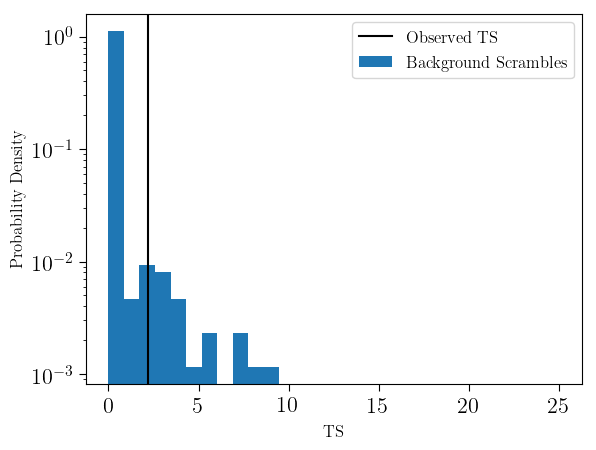
\includegraphics[width=0.9\textwidth]{/data/condor_builds/users/efried/FastResponseAnalysis/trunk/2017_01_01_Fast_Response_Example/TS_distribution.png}}
\newcommand{\upperlim}{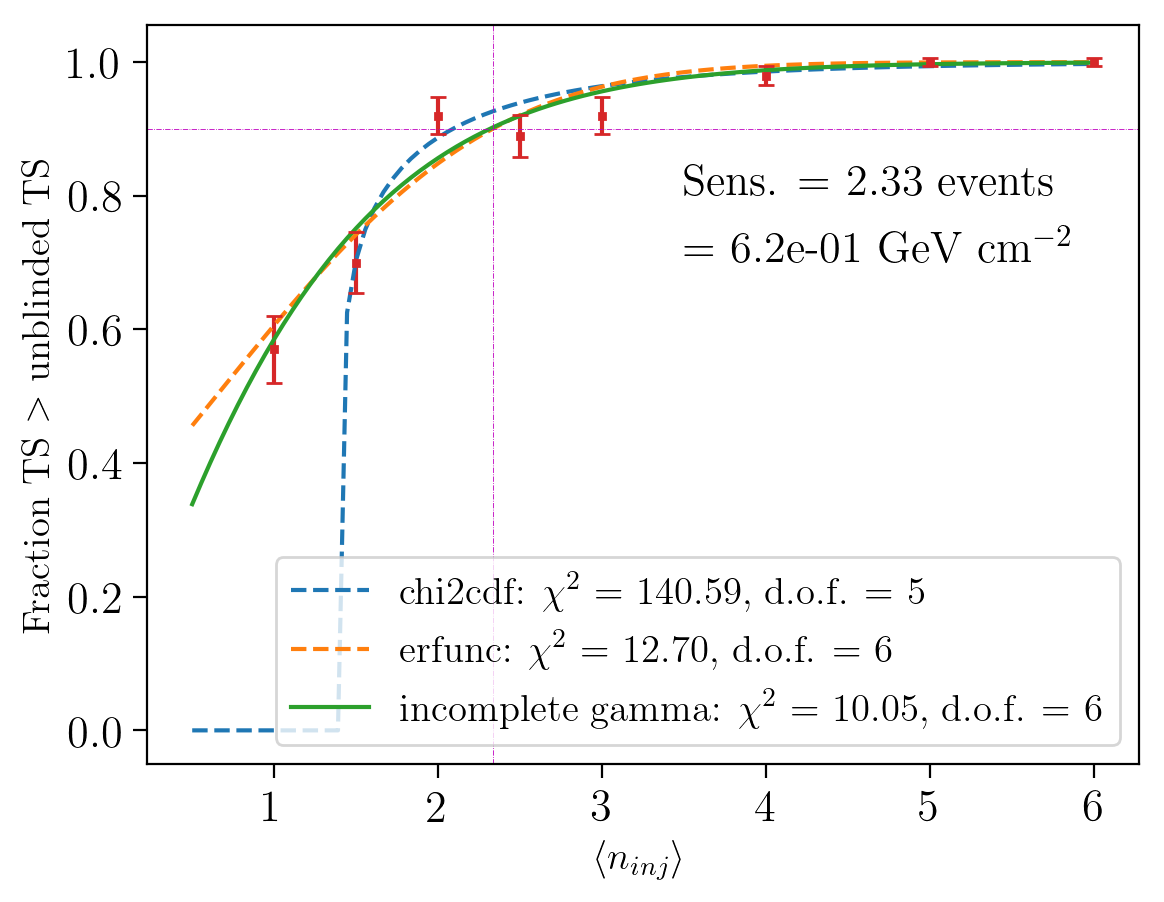
\includegraphics[width=0.9\textwidth]{/data/condor_builds/users/efried/FastResponseAnalysis/trunk/2017_01_01_Fast_Response_Example/upper_limit_distribution.png}}
\newcommand{\nsscan}{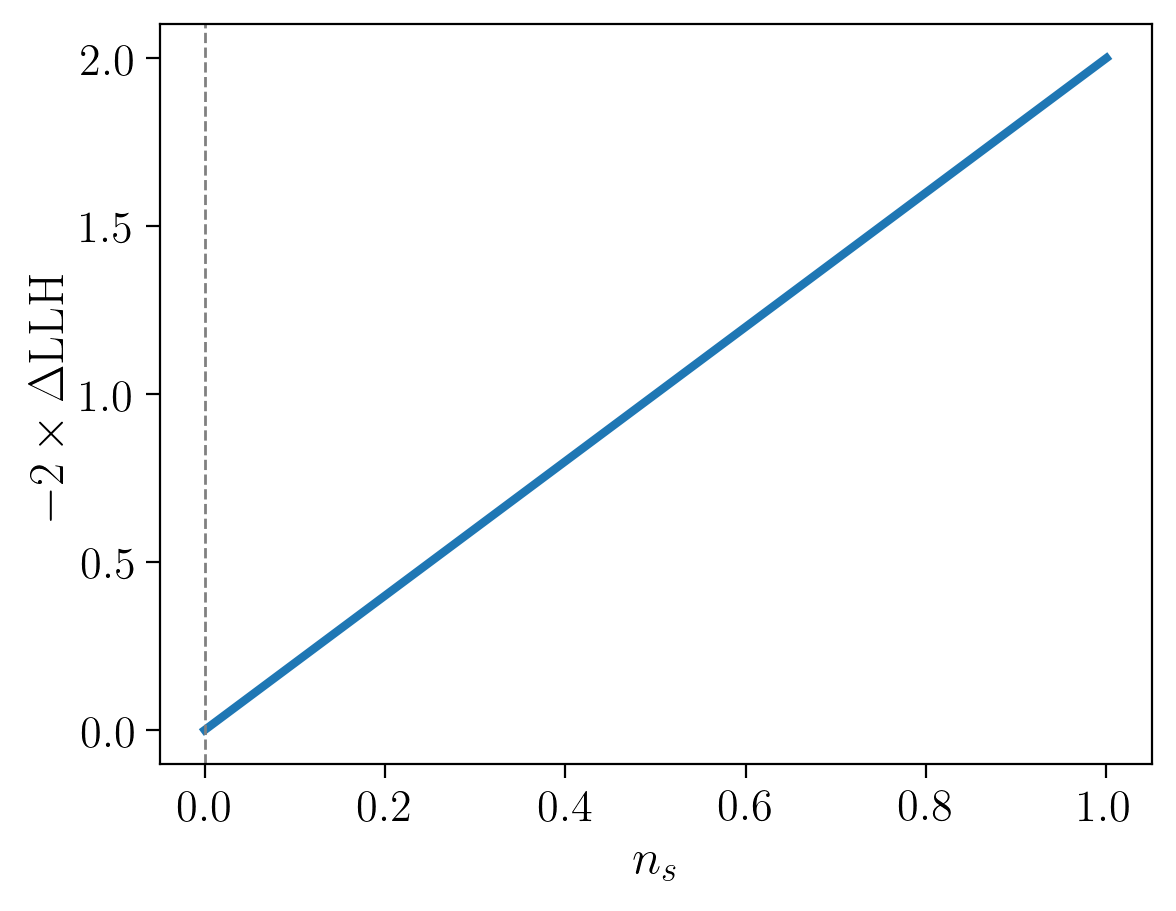
\includegraphics[width=0.9\textwidth]{/data/condor_builds/users/efried/FastResponseAnalysis/trunk/2017_01_01_Fast_Response_Example/llh_ns_scan.png}}
\newcommand{\obsdate}{2017-01-01 -- 2017-01-02}
\newcommand{\multiplicity}{/data/condor_builds/users/efried/FastResponseAnalysis/trunk/2017_01_01_Fast_Response_Example/IN_ICE_SIMPLE_MULTIPLICITY_plot.png}
\newcommand{\survivialfunctionplot}{}
\newcommand{\backgroundpdfplot}{}
\newcommand{\sourcetable}{
\begin{longtable}{ll}
\hline
Source Name & Fast Response Example\\
Trigger Time & 2017-01-02 00:00:00.000 (MJD=57755.000000)\\
Start Time & 2017-01-01 12:00:00.000 (Trigger-43200.0s)\\
Stop Time & 2017-01-02 12:00:00.000 (Trigger+43200.0s)\\
Time Window & 86400.0s\\
\hline
\end{longtable}}
\newcommand{\skylabtable}{
\begin{longtable}{ll}
\hline
Skylab Version & 2.7.2\\
IceTray Path & ['/data/condor\_builds/users/efried/icerec/build\_realtime/lib/icecube/icetray']\\
Created by & i3home/efried\\
Dataset Used & gfu online/version-001-p01/\\
Dataset details & Real-time Gamma-Ray Follow-Up (GFU) Sample with leap second bug fix and official\\
 & neutrino sources format.\\
\hline
\end{longtable}}
\newcommand{\runtimetable}{
\begin{longtable}{lllll}
\hline
Run & Start Time & Stop Time & Duration & Livetime\\ \hline
129004 & 2017-01-01 00:08:05 & 2017-01-01 08:07:31 & 7:59:26 & 0.0s\\
129005 & 2017-01-01 08:07:31 & 2017-01-01 16:07:42 & 8:00:11 & 14862.0s\\
129006 & 2017-01-01 16:07:42 & 2017-01-02 00:07:57 & 8:00:14 & 28815.0s\\
129007 & 2017-01-02 00:07:57 & 2017-01-02 08:08:11 & 8:00:14 & 28814.0s\\
129008 & 2017-01-02 08:09:17 & 2017-01-02 16:08:42 & 7:59:25 & 13843.0s\\
129009 & 2017-01-02 16:08:42 & 2017-01-03 00:08:48 & 8:00:05 & 0.0s\\
\hline
\end{longtable}}
\newcommand{\runstatustable}{
\begin{longtable}{lllllll}
\hline
Run & Status & Light & Filter Mode & Run Mode & OK & GFU\\ \hline
129004 & SUCCESS & dark & PhysicsFiltering & PhysicsTrig & OK & 0.0\\
129005 & SUCCESS & dark & PhysicsFiltering & PhysicsTrig & OK & 0.0\\
129006 & SUCCESS & dark & PhysicsFiltering & PhysicsTrig & OK & 0.0\\
129007 & SUCCESS & dark & PhysicsFiltering & PhysicsTrig & OK & 0.0\\
129008 & SUCCESS & dark & PhysicsFiltering & PhysicsTrig & OK & 0.0\\
129009 & SUCCESS & dark & PhysicsFiltering & PhysicsTrig & OK & 0.0\\
\hline
\end{longtable}}
\newcommand{\livetime}{86,334.0}
\newcommand{\ontimetable}{
\begin{longtable}{ll}
\hline
Access Method & database\\
Stream & \texttt{neutrino16}\\
Query Time & 2020-08-20 17:39:23\\
Start Time & 2017-01-01 00:08:05\\
Stop Time & 2017-01-03 00:08:48\\
\hline
\end{longtable}}
\newcommand{\event}{
\begin{longtable}{ll}
\hline
Run:Event & 129006:19236235\\
Time & 57754.74787590005\\
$\alpha$, $\delta$ & 249.38\degree, -45.84\degree\\
Angular Uncertainty (90\%) & 0.70\degree\\
Distance from Source & 0.94\degree\\
Reconstructed Energy (GeV) & 3.34e+05\\
Spatial Weight & 1760.04\\
Energy Weight & 2.38\\
\hline
\end{longtable}}
\newcommand{\results}{
\begin{longtable}{ll}
\hline
$n_s$ & 0.860\\
$TS$ & 2.208\\
$p-value$ & 0.0240\\
\hline
\end{longtable}}
